\documentclass{article}

\usepackage{generalsnips}
\usepackage{calculussnips}
\usepackage[margin = 1in]{geometry}
\usepackage{pdfpages}
\usepackage[spanish]{babel}
\usepackage{amsmath}
\usepackage{amsthm}
\usepackage[utf8]{inputenc}
\usepackage{titlesec}
\usepackage{xpatch}
\usepackage{fancyhdr}
\usepackage{tikz}
\usepackage{hyperref}
\usepackage{enumitem}
\usepackage{float}
\usepackage{wrapfig}


\begin{document}
\begin{titlepage}

    \title{}
    
\end{titlepage}


\begin{titlepage}
    \begin{center}
        \thispagestyle{empty}
        \renewcommand{\headrulewidth}{0pt}
        \renewcommand{\footrulewidth}{0pt}
        
        \begin{tabular}{ p{0.5\textwidth}p{0.5\textwidth} }
            \begin{flushleft}
                Facultad de Ciencias Económicas \\
                Universidad Francisco Marroquín \\
                Administración Financiera I \\ 
                Catedrático: Ana Del Carmen Muñoz Del Valle \\ 
                Auxiliar: Edwin Adalberto Calderón Cárdenas \\
                Guatemala \\
                07 de septiembre 2020 \\ 
            \end{flushleft}
            &
            \begin{flushright}
                
\includegraphics[width=0.5\textwidth]{ufmlogo.png} \\ 
            \end{flushright} \\ 
        \end{tabular}
        
            
        \cfoot{} % this is to remove the page number
        \vspace*{7cm}
        {
            \Huge Parte Teórica Parcial \#1 - Administración Financiera I
        }
 
        \vspace{1.5cm}

 
        \vfill
             
        \vspace{0.8cm}
        
        
        \begin{flushleft}
            \begin{tabular}{ ll }
                David Corzo      & 20190432 \\
                Daniel Cabrera   & 20190069 \\
            \end{tabular}
        \end{flushleft}     
    \end{center}
\end{titlepage}

%%%%%%%%%%%%%%%%%%%%%%%%%%%%%%%%%%%%%%%%%%%%%%%%%%%%%%%%%%%%%%%%%%%%%%%%%%%%%%%%%%%%%%%%%%%%%%%%%%%%%%%%%%%%%%%%%%%%%%%%%%%%%%%%%%%%%%%%%%%%%%

\section{Introducción}
{
    Las razones de manejo de activos tienen una función sumamente importante dentro del análisis de la empresa. Dichas razones indican qué tan efectiva está siendo la empresa para manejar sus activos. Un mal uso de activos en la empresa puede significar potenciales pérdidas e incluso quiebra de la empresa en cuestión, es por eso inmanente tener en cuenta estas razones a la hora de analizar la empresa, ya sea propia o de terceros. Basado en las razones promedio de la industria, se comparan las razones particulares de dicha empresa para poder determinar si están altas o bajas. En ocasiones se desean que estén altas y en otras ocasiones se desea que estén bajas. En síntesis lo que buscan resolver estas poderosas e innovadoras herramientas es dar una respuesta a la pregunta ¿los datos pertinentes al activo reportados en el balance general se ven razonables? si se ven atípicos, ¿es normal en esta industria? Tener mala gestión y manejo en activos puede ocasionar bajas en las ventas, menores utilidades y menor eficiencia a la hora de producir. Dichas razones se dividen en:
    \begin{itemize}
        \item Rotación de inventario.
        \item Días de rotación de inventario.
        \item Rotación de cartera.
        \item Días pendientes de cobro
        \item Rotación de activos fijos netos.
        \item Rotación de activos totales.
    \end{itemize}
}

\subsection{Rotación de inventario. Días de rotación de inventario.}
La razón de la rotación de inventario nos dice la actividad de inventario que tiene la empresa, lo que indica en general, es cuántas veces las existencias totales en inventario se han renovado en un tiempo generalmente de un año. Típicamente esta razón se compara con datos históricos de la misma empresa o con otras empresas en la misma industria. La razón de días de rotación de inventario indica cuántos días cada cuántos días se renueva el inventario. En breve, la rotación de los inventarios indica cuántas veces en el año se ha renovado el inventario y los días de rotación de inventarios indica cada cuántos días se renueva el inventario. 
\par 
A continuación la fórmula para calcular la rotación de inventarios y días pendientes de rotación de inventarios.
\begin{center}
   \begin{align*}
       \text{ Rotación de inventarios } &= \frac{\text{ Costo de ventas }}{ \text{ Inventario } } \\ \\ 
       \text{ Días de rotación de inventario } &= \frac{\text{ Inventario }}{ \p{\cfrac{\text{ Costo de ventas }}{365}} } \\ 
   \end{align*}
\end{center}


\subsection{Rotación de cartera. Días pendientes de cobro.}
La razón de rotación de cartera nos dice la frecuencia con la cual se está recolectando las cuentas por cobrar o se cobran las deudas a acreedores, si esta resulta baja la empresa puede estar en riesgo de insolvencia a corto plazo, en general se desea que esta razón sea lo más alta posible. Los días pendientes de cobro nos dice en promedio cada cuantos días la empresa colecta cuentas por cobrar. 
\par
A continuación la fórmula para calcular la Rotación de cartera \& Días pendientes de cobro.
\begin{center}
   \begin{align*}
       \text{ Rotación de cartera } &= \frac{\text{ Ventas }}{\text{ Cuentas por cobrar }} 
       \\ \\ 
       \text{ Días pendientes de cobro } &= \frac{\text{ Cuentas por cobrar  }}{\cfrac{\text{ Ventas }}{365}} 
       \\ 
   \end{align*}
\end{center}

\subsection{Rotación de activos fijos.}
La rotación de activos fijos nos indica qué tan bien la empresa está empleando sus activos fijos tales como propiedad, planta y equipo en generar ventas. Para medir qué tan efectivo es la utilización de dichos activos. Para motivos de maximización de beneficio, esta razón en general siempre se desea lo más alta posible, ya que es deseable ser eficiente en el empleo de activos fijos y así poder generar más utilidades. \par 
A continuación se presentan la fórmula para el cálculo de la razón de rotación de activo fijos.
\begin{center}
   \begin{align*}
       \text{ Rotación de activos fijos } = \frac{\text{ Ventas }}{\text{ Activos fijos netos }} \\
   \end{align*}
\end{center}

\subsection{Rotación de activos totales.}
La rotación de activos totales nos indica qué tan bien la empresa está empleando todos sus activos en función de generar ventas. Nos proporciona un análisis de la situación financiera de la empresa sobre el nivel de eficiencia con la cual la empresa hace uso de sus recursos con el objetivo de generar ventas.
\begin{center}
   \begin{align*}
       \text{ Rotación de activos totales. } = \frac{\text{ Ventas }}{\text{ Activos totales }} \\
   \end{align*}
\end{center}

\section{Ejemplo \# 1}
\begin{center}
    \begin{figure}[H]
        \centering
        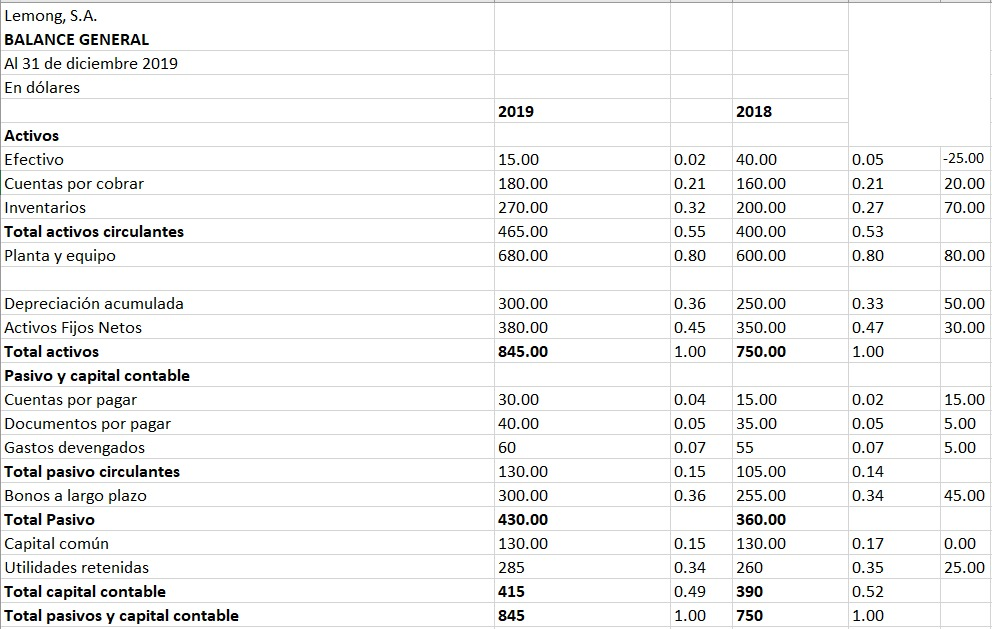
\includegraphics[width=\textwidth]{bg.jpeg}
    \end{figure}
    \begin{figure}[H]
        \centering
        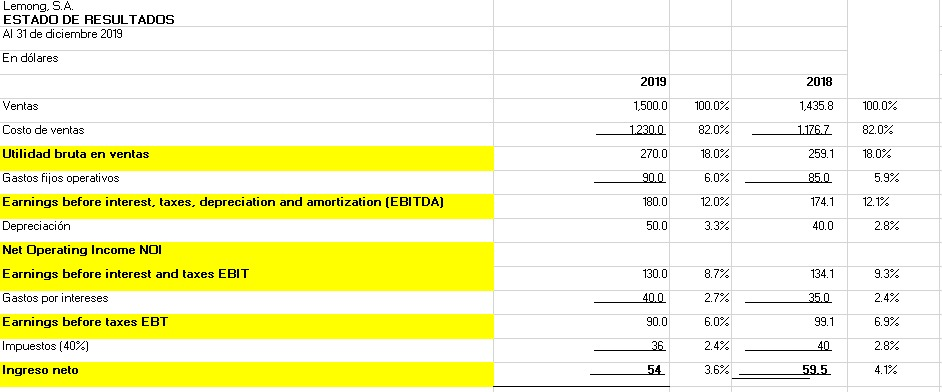
\includegraphics[width=\textwidth]{er.jpeg}
    \end{figure}
\end{center}
\newpage
\begin{wrapfigure}{r}{0.6\textwidth}
    \begin{center}
        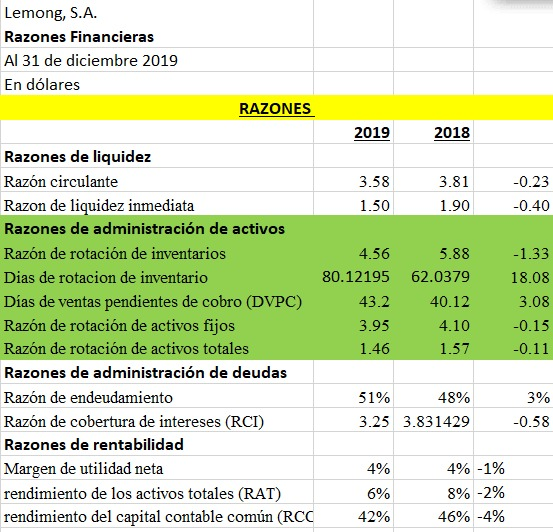
\includegraphics[width=0.6\textwidth]{rf.jpeg}
    \end{center}
\end{wrapfigure}

En este ejemplo se hace la comparación de las razones financieras de la empresa Lemong, S.A. entre el año 2018 y 2019, en este caso en particular a pesar que no se tiene información de la industria en la que Lemong opera, las razones nos brindan información fundamental, como podemos observar en la figura nos proporciona información pertinente al empleo de activos totales, activos fijos al igual que información de cómo se está rotando el inventario y con qué frecuencia. Si analizamos dichas razones podemos encontrar un cambio en la rotación de inventarios, el cual pasó de ser cada 62 días a ser cada 80 días, esto puede significar que la mercadería en inventario esté dañada o que hayan cambiado las preferencias de los consumidores. En cuanto a los días pendientes de cobro, podemos afirmar de nuevo que hay una baja en el inventario, puesto a que se mantuvo constante durante los dos años, indicando que hay un retardo en la colecta de cuentas por cobrar manteniéndose entre 43 a 40 días, lo cual pone a la empresa Lemong en peligro de insolvencia (dependiendo la industria). Dado que no tenemos suficiente información de la industria en la que Lemong opera, se pueden derivar ‘corolarios’ acerca de la industria, por ejemplo, el hecho que las razones días pendientes de cobro, días de rotación de inventario y rotación de inventario, hayan salido tan atípicas indica que una de dos cosas, o la empresa ha tenido muy malas ventas o pocas ventas es lo normal en esta industria, puede que esté en una industria que se dedique a productos de lujo o inmuebles donde estas razones salen normalmente más anormales a comparación de otras industrias.

\newpage
\section{Ejemplo \#2}
\begin{figure}[H]
    \centering
    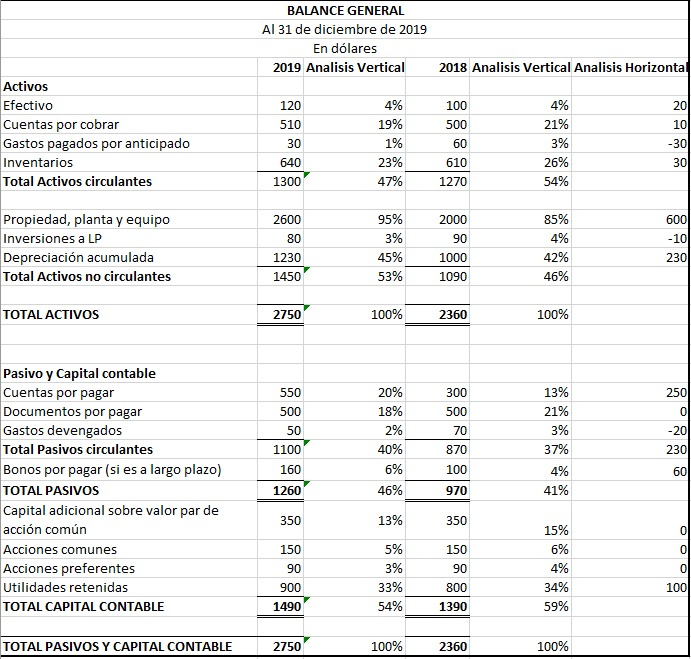
\includegraphics[width=0.8\textwidth]{bg1.jpeg}
\end{figure}
\begin{figure}[H]
    \centering
    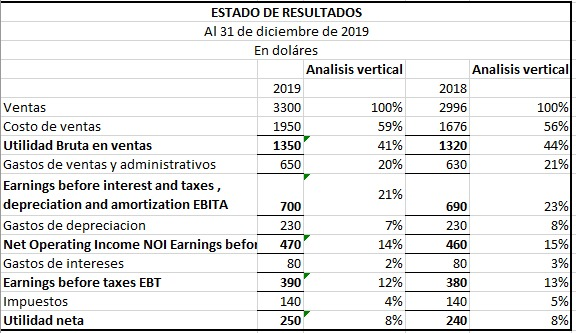
\includegraphics[width=0.8\textwidth]{er1.jpeg}
\end{figure}

\begin{wrapfigure}{r}{0.6\textwidth}
    \begin{center}
        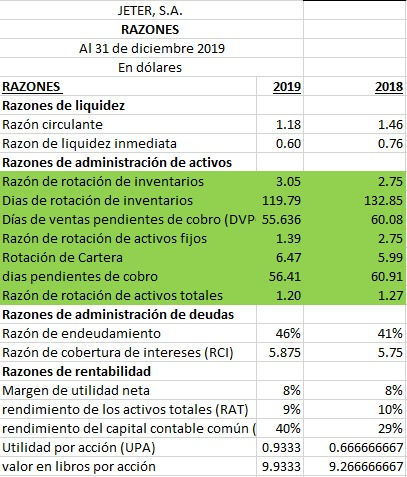
\includegraphics[width=0.6\textwidth]{rf1.jpeg}
    \end{center}
\end{wrapfigure}
Como podemos observar en el ejemplo anteriormente presentado, la razón de rotación de inventario se encuentra en un promedio de 3 veces al año, lo cual puede significar bajo movimiento según la industria en la que opere. Por otro lado, como podemos ver ha disminuido marginalmente los días de cobro, lo cual indica una mejora, ya que significa que están vendiendo mayores cantidades. 
En cuanto a la rotación de activos fijos, podemos ver que cambiaron casi dos veces al año lo cual representa baja marginal pero no significativa. 
\par 
En cuanto a la rotación de cartera podemos ver que aumentó en 2019, eso significa que se alentó la frecuencia con la cual colectan las cuentas por cobrar, esto puede significar un posible riesgo puesto a que la empresa puede tener problemas de solvencia. \par 


\section{Conclusión}
En conclusión las razones financieras son una herramienta muy poderosa que uno como empresario y/o contador debe emplear para hacer inteligente uso de sus recursos y poder medir sus objetivos, al igual que detectar problemas y poder resolverlos. \par Esto también nos sirve como inversionistas para poder hacer inteligentes y acertadas inversiones en empresas que posean salud y resiliencia.

\onecolumn



{
\newpage
\section*{Bibliografía}
\begin{enumerate}[label={[\arabic*]}]
    \item Essentials of Managerial Finance by Scott Besley \& Eugene F. Brigham, Cap.2, pg.54-56.
\end{enumerate}
}
%%%%%%%%%%%%%%%%%%%%%%%%%%%%%%%%%%%%%%%%%%%%%%%%%%%%%%%%%%%%%%%%%%%%%%%%%%%%%%%%%%%%%%%%%%%%%%%%%%%%%%%%%%%%%%%%%%%%%%%%%%%%%%%%%%%%%%%%%%%%%%
\end{document}

